\paragraph*{Datová obfuskace}
%https://researchspace.auckland.ac.nz/bitstream/handle/2292/3491/TR148.pdf¨
%https://www.paladion.net/blogs/code-obfuscation-part-2-obfuscating-data-structures
%https://medium.com/better-programming/code-obfuscation-introduction-to-code-obfuscation-part-1-93a6797349b0
%https://selab.fbk.eu/ceccato/papers/2015/spro2015.pdf

Metoda datové obfuskace pracuje s maskováním datových struktur pomocí jejich přeměny na jiné sémanticky však stejné. Tento druh obfuskace se často používá pro skrytí citlivých informací. V případě malwaru se může jednat o důležité informace jako například doménové jméno či IP adresy CnC serveru, šifrovací klíče apod. Tyto transformace mohou být provedeny několika způsoby a jsou popsány níže \cite{DataObfuscation}.

\subparagraph*{Nahrazení statických dat}
%% Změna datových struktur
%% převod proměnných na metody
%% globalizace

Nejjednodušší způsob obfuskace statických dat je nahrazení metodou. Data jsou nahrazena kódem, který je bude dynamicky generovat. Účinnost tohoto řešení se zvyšuje s počtem volaných funkcí, jejichž volání je náhodně rozloženo do toku programu \cite{DataObfuscation}. Pro zmatení reverzního inženýra je možné přidat také několik výstupů, ke kterým při~normálním běhu programu nedojde.

Tuto metodu lze vidět na následující ukázce č. \ref{src:StaticData}. Statická data byla nahrazena jednoduchým \emph{switchem}, který podle čísla vstupu vrátí požadovanou hodnotu.

\noindent
\begin{minipage}[t]{1\textwidth}
    \lstinputlisting[basicstyle=\footnotesize,caption={Generování statických dat},label=src:StaticData]{zdrojaky/obfuskace/staticka-data.cs}
\end{minipage}

\subparagraph*{Rozdělení proměnných}
%% Změna z a=123 na a = 100 ; b = 20; c = 3 ; a + b + c 

Velmi účinnou technikou obfuskace proměnných je jejich rozdělení a to nejlépe za použití různých datových typů \cite{DataObfuscation2}. Cílem je zmást reverzního inženýra velkým množstvím použitých proměnných. \par Síla a odolnost této transformace roste s počtem použitých proměnných a různorodosti jejich typů.

Následující ukázka kódu č. \ref{src:VariableJoining1} a \ref{src:VariableJoining2} prezentuje tuto metodu. Původní proměnnou je možné vidět v prvním výpisu č. \ref{src:VariableJoining1} obfuskvanou proměnnou pak v ukázce č. \ref{src:VariableJoining2}. Pokud bychom definice proměnných proložili sekvencemi vykonávaného kódu docílili bychom ještě lepšího výsledku.

%\ref{ref:SkladaniPromenne}

%%%%%%%%%%%%%%% Výstup %%%%%%%%%%%%%
%\begin{center}	
    %\label{src:SkladaniPromenne}
    \noindent
    \begin{minipage}[t]{1\textwidth}
        \noindent
        \centering
        \lstinputlisting[basicstyle=\footnotesize,caption={Proměnná bez obfuskace},label=src:VariableJoining1]{zdrojaky/obfuskace/skladani-promenne1.cs}
    \end{minipage}
    \newline
    %\hfill
    \begin{minipage}[t]{1\textwidth}
        \lstinputlisting[basicstyle=\footnotesize,caption={Obfuskovaná proměnná},label=src:VariableJoining2]{zdrojaky/obfuskace/skladani-promenne2.cs}
    \end{minipage}
%\end{center}
%%%%%%%%%%%%%%%%%%%%%%%%%%%%%%%%%%%%%%


\subparagraph*{Globalizace proměnné}
%%% TODO
Máme-li funkce, například FA() a FB(), jež používají stejnou lokální proměnnou, definovanou ve svém těle a nevykonávají-li se souběžně, můžeme takovouto proměnnou deklarovat globálně a bude tak sdílena mezi oběma funkcemi \cite{DataObfuscation}. 

\subparagraph*{Sloučení proměnných}
%% sloučení více proměnných do jedné třeba 2 32b čísla mohou být jako 64b

Další metodou obfuskace proměnných je jejich sloučení do jedné. Příkladem mohou být dvě 32-bitová čísla X a Y. Tato čísla mohou být sloučena do jednoho 64-bitového dle následujícího vzorce \ref{src:SlouceniPromennychDo64b} \cite{DataObfuscation}.

\begin{equation}
    \label{src:SlouceniPromennychDo64b}
    V = 2^{32} * Y + X
\end{equation}

Odolnost této přeměny je malá, protože deobfuskátor může odhadnout, že proměnná~V se skládá ze dvou proměnných a to zkoumáním aritmetických operací.


\subparagraph*{Šifrování a kódování}
%% TODO
%% Zašifruji data
%%https://medium.com/@bromiley/malware-monday-obfuscation-f65239146db0

Další možností obfuskace dat je jejich šifrování popřípadě jejich kódování. Šifrovány mohou být buď jednotlivé části kódu nebo celé sekce spustitelného souboru \cite{sevagas_2014}. Zašifrovaná data jsou následně při spuštění dešifrována \cite{guardsquare_2019}. Tím je zaručeno, že program funguje tak jak byl vytvořen.

Často je možné se setkat s šifrováním pomocí bitové funkce \emph{XOR} nebo kódováním do \emph{Base64}. Takovéto zakrytí dat může oddálit odhalení skutečného obsahu, protože nemusí být na první pohled patrné, že jsou data šifrována nebo kódována.


%Oproti šifrování, užívaném například v síťové komunikaci, se používají také často již prolomené šifry. 
%Můžeme se setkat s šifrováním pomocí bitové funkce XOR nebo kódovaní do Base64. Takovéto zakrytí dat může prodloužit odhalení skutečného obsahu, protože při spuštění se kód prvně dešifruje a 

        %http://www.hjp.at/doc/rfc/rfc4648.html#sec_4
        %https://iopscience.iop.org/article/10.1088/1742-6596/1007/1/012003/pdf
        
        
Kódování \emph{Base64} bylo původně navrženo pro přenos příloh v emailové komunikaci a je~součásti standardu MIME \cite{sikorski2012practical}. Kódování \emph{Base64} umožňuje převést binární data na ASCII řetězec~a, jak~značí číslo 64 v názvu kódování, používá se právě 64 (resp. 65) znaků US-ASCII. Znaky užívané kódováním jsou a-z, A-Z, 0-9, +, / a = pro zarovnání délky \cite{RFC4648}.

Implementace do vlastního programu je velmi jednoduchá a většina moderních programovacích jazyků už toto kódování umožňuje. Útočnici (autoři malwaru) tak často využívají toto kódování ke skrytí závadného kódu nebo dat. 

%check this:
%Kódování pomocí Base64 umožňuje převést binární data na ASCII řetězec. Tím pádem lze přenést binární data jakoukoliv cestou. Původně bylo navrženo pro přenos příloh v emailové komunikaci. 

% komplikuje to zjištění co je obsahem
% umožňuje použít vlastní abecedu
% má popsaný algoritmus přesně (RFC)
% 

Šifrování pomocí exkluzivní disjunkce (\emph{XOR}) je velmi oblíbeným způsobem šifrováním mezi tvůrci malwaru \cite{sikorski2012practical}, protože se jedná o oboustrannou funkci, není potřeba implementovat různé algoritmy pro šifrování a dešifrování \ref{fig:XorSifrovani}. Klíčem je vždy proud bitů \cite{kpb_ochodkova2019}.

\begin{figure}[!ht]
    \caption{De/šifrování pomocí XOR}
    \centering
    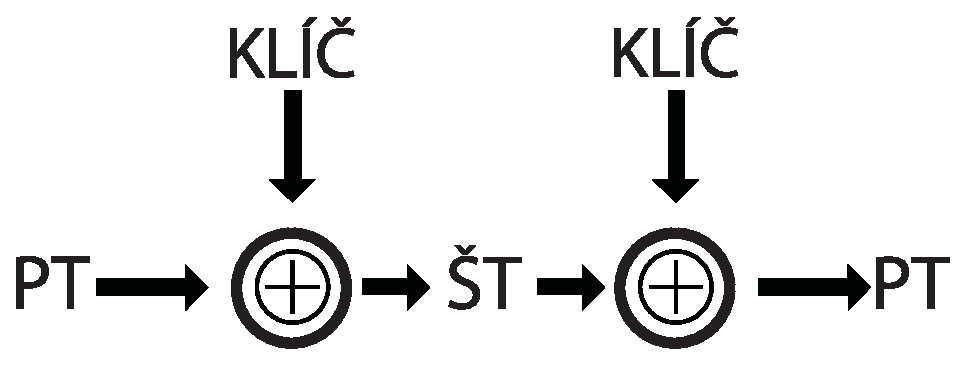
\includegraphics[width=75mm,scale=0.5]{Figures/obrazky/pt-st-pt-xorsifra.eps}
    \label{fig:XorSifrovani}
\end{figure}
    
%Šifrování pomocí exkluzivní disjunkce je velmi jednoduché na implementaci a protože se jedná o oboustrannou funkci, odpadá nutnost impl. Klíčem je vždy proud bitů. 
 
 
 
 % oboustranná funkce P -> C -> P